\subsection{Cadmiumsulfid (CdS)}
Cadmiumsulfid ist genau wie ZnO ein direkter $\text{II}^\text{b}$-VI Verbindungshalbleiter und kristallisiert in unter Normalbedingungen meist in hexagonaler Wurzit-Struktur ($\upalpha$-Cadmiumsulfid), die sich als energetisch günstiger erweist, kann aber unter hohen Drücken auch in der kubischen Zinkblende-Struktur ($\upbeta$-Cadmiumsulfid) entstehen. Die Gitterkonstanten der zumeist vorliegenden Wurzit-Struktur betragen $\text{a} = \text{b} = 4.138 \AA$ und $\text{c} = 6.718 \AA$ \cite{Hotje.2003}. Auch hier erfolgt eine Aufspaltung in drei Subbänder (A, B und C) mit den Bandlücken $\text{E}_\text{g}= 2.582$ eV, $\Updelta\text{E}_\text{AB}= 16$ meV und $\Updelta \text{E}_\text{BC}= 57$ meV \cite{Thomas.1962}. Wobei auch hier die Übergänge der Valenzbänder zum Leitungsband den Auswahlregeln analog zum ZnO entsprechen. Der Übergang vom $\text{VB}_\text{A}$ zum Leitungsband ist nur bei einem elektrischen Feldvektor $\vec{\textbf{E}}$ senkrecht zum Gittervektor $\vec{\textbf{c}}$  ($\vec{\textbf{E}} \bot \vec{\textbf{c}}$) möglich, die beiden anderen Übergänge funktionieren sowohl bei $\vec{\textbf{E}} \bot \vec{\textbf{c}}$ als auch $\vec{\textbf{E}} \| \vec{\textbf{c}}$. Diese Dipolauswahlregel ist aber nicht streng, sodass trotzdem ein schwacher Übergang zum $\text{VB}_A$ bei  $\vec{\textbf{E}} \| \vec{\textbf{c}}$ zu beobachten ist \cite{Thomas.1962}. Bei CdS formen die leeren 5s-Orbitale des Cadmium (Cd) das Leitungsband, während die komplett gefüllten 3p-Orbitale des Schwefels (S) das Valenzband formen. Auch hat die Bindung aufgrund des Elektronegativitätsunterschieds von $\approx 1$ einen hohen ionischen Anteil. Die Brechungsindizes belaufen sich auf $\text{n}_\text{o}= 2.726$ und $\text{n}_\text{ao}= 2.743$ für $\uplambda= 515$ nm respektive $\text{E}_\text{Photon}= 2,407$ eV bei Raumtemperatur – die Dispersion beträgt bei selbiger Wellenlänge $\partial$n/$\partial \uplambda\approx -8.8460 \upmu \text{m}^\text{-1}$ \cite{Bieniewski.1963}

%Zeile26
Für ZnO ($\text{a}_\text{b}= 1.8$ nm \cite{Haranath.2009} gegen $\text{c}= 0.52$ nm) und CdS ($\text{a}_\text{b}= 2.8$ nm \cite{Titova.2006} gegen $\text{c} = 0.67$ nm) ist dies jeweils erfüllt.
%Zeile 33
Für ZnO und CdS ergeben sich die Bindungsenergien zu $\text{E}_\text{X,ZnO}=$ 49...63 meV \cite{Mang.1995} und $\text{E}_\text{X,CdS}= 27..31$ meV \cite{Imada.2002} bei $\text{n}_\text{B}= 1$ für die drei Subbänder A, B und C, die Lebensdauer liegt im typischerweise Bereich von 10$^\text{-10}$ bis 10$^\text{-6}$ Sekunden.
\section{Der Vapour-Liquid-Solid Mechanismus}
\label{VLS}
Der Vapour-Liquid-Solid Mechanismus (kurz \textit{VLS}) nach Wagner und Ellis (1964) \cite{Wagner.1964} ist eine Methode zur Herstellung von Nanodrähten (engl. \textit{nanowire}, kurz \textit{NW}). Das zugrundeliegende Prinzip dieser Methode ist ein, durch einen Katalysator vermitteltes, eindimensionales Strukturwachstum. Hierbei dient der Katalysator, in diesem Fall Gold, als symmetriebrechendes Element, das eine Wachstumsrichtung stark gegenüber den anderen bevorzugt. Hierzu wird auf das Wachstumssubstrat eine dünne Schicht Gold aufgsputtert und aufgeschmolzen – es formen sich unter dem Einfluss der Oberflächenspannung kleine Goldtropfen. Der Durchmesser dieser Tropfen reicht von einigen zehn Nanometern bis hin zu einigen Mikrometern und hängt stark von der ursprünglichen Schichtdicke des Goldes ab. Wird nun das Wachstumsmaterial in der Gasphase zugeführt, adsorbiert es vorzugsweise an der Oberfläche dieser flüssigen Goldtropfen. Mit fortschreitender Adsorption erreicht das Wachstumsmaterial in den Goldtropfen eine Übersättigung in deren Folge es an der Grenzfläche zum Substrat auskristallisiert, da hier die aufzuwendende Oberflächenenergie am geringsten ist. Im weiteren Verlauf scheidet sich immer mehr Material unter dem Goldtropfen ab, sodass die Struktur mit dem Goldtropfen an der Spitze weiter und weiter in die Höhe wächst – es bilden sich dünne, einkristalline Nanodrähte, deren Höhe maßgeblich von der Dauer des Materialstroms bestimmt wird.\\
Parallel hierzu findet ein als Vapour-Solid (kurz \textit{VS}) benannter Ablagerungsprozess statt. Dieser sorgt dafür, dass sich das Wachstumsmaterial auch an die Seitenflächen der Nanodrähte anlagern, es entstehen segelförmige Auswüchse an den Nanodrähten. Dennoch wird der Durchmesser der Drähte weiterhin primär vom Durchmesser der Goldtropfen bestimmt, da der VS-Prozess verglichen mit dem VLS-Prozess um Größenordnungen langsamer verläuft \cite{Geburt.Diss}.

\subsubsection{Störstellen}
Exzitonen neigen, vor allem bei geringen Temperaturen, dazu sich an Störstellen im Kristallgitter zu lokalisieren, da sie hier ein energetischen Minimum einnehmen können. Ihre Energie reduziert sich entsprechend der Bindungsenergie dieses Komplexes aus Störstelle und Exziton. Die Bindungsenergie ist abhängig von der Art der Störstelle und rangiert für Donatoren in ZnO typischerweise von $15..20$ meV \cite{Meyer.2004}. Als Störstellen im Kristall können intrinsische Gitterdefekte wie bspw. Leerstellen und Zwischengitteratome, als auch extrinsische Defekte , wie eingebrachte Fremdatome, wirken. Weitere mehrdimensionale Gitterfehler sind unter anderem Stapelfehler, Versetzungen oder gar Poren im Material, die eine starke Verzerrung der Bandlücke im umliegenden Bereich erzeugen.  Man unterscheidet zwischen Exzitonen, die an neutrale Donatoren (\textit{D$^\text{0}$X}), an ionisierte Donatoren (\textit{D$^\text{+}$X}), an neutrale Akzeptoren (\textit{A$^\text{0}$X}) oder an geladene Akzeptoren (\textit{A$^\text{-}$X}) gebunden sind. Hierbei ist der A$^\text{0}$X-Zustand der stabilste, gefolgt vom D$^\text{0}$X und dem D$^\text{+}$X-Zustand, der letzter Komplex A$^\text{-}$X ist instabil und zerfällt in ein Elektron sowie ein neutralen Akzeptor, da dies einen energetisch günstigeren Zustand darstellt \cite{Klingshirn.2007}. Beide Materialsysteme, sowohl ZnO als auch CdS, die in dieser Thesis betrachtet werden, zeigen ein intrinsisches n-leitendes Verhalten, entsprechend oft treten Donatoren als Störstellen auf \cite{Ozgur.2005}, bei tiefen Temperaturen dominiert also die D$^\text{0}$X-Linie. Gebundene Exzitonen besitzen keine kinetische Energie bzgl. ihrer Schwerpunktbewegung, in Bereichen tiefer Temperaturen sind folglich ihre Rekombinationslinien sehr scharf, verglichen mit denen der freien Exzitonen. Generell lässt sich zur Exzitonen-Rekombination an einem Donator sagen, dass das Exziton ein Teil der freiwerdenden Energie an ein Elektron dieses Donators abgeben kann, sodass der Donator angeregt oder sogar ionisiert wird – das emittierte Photon ist also in seiner Energie nach unten verschoben. Man unterscheidet im allgemeinen \textit{flache} und \textit{tiefe Störstellen}. Flache Störstellen sind dadurch gekennzeichnet, dass die Donatoren energetisch knapp unterhalb der Leistungsbandkante, die Akzeptoren knapp überhalb der Valenzbandkante liegen, tiefe Störstellen liegen hingegen weit innerhalb der Bandlücke. Sie bilden ein Defektband aus, das Lumineszenz schon bei Anregungen deutlich kleiner der Bandlücke erlaubt. Aufgrund vieler Überlagerungen mit Phononrepliken weist diese (engl. \textit{deep-level-emission}, kurz \textit{DLE}) verglichen mit der Bandkanten-nahe Emission (engl. \textit{near band gap emission}, kurz \textit{NBE}) eine sehr große Halbwertsbreite auf. Die DLE setzt sich aus Überlagerungen vieler verschiedener Lumineszenzbanden zusammen, die ihren jeweiligen Ursprung in den verschiedenen Defektarten haben. Bei zunehmenden Anregungsintensitäten sättigt die DLE ab, es nimmt nur die NBE weiter zu.

\subsubsection{Oberflächenexzitonen}
Bei kleinen Strukturen, zu denen Nanodrähte zählen, ergibt sich ein großes relatives Verhältnis von Oberfläche zu Volumen. Entsprechend groß ist die Chance ein Exziton dort zu finden. Obwohl sich die Nanodrähte elektronisch ähnlich verhalten wie ihr Volumenmaterial (engl. \textit{bulkmaterial}), weisen sie doch optische Unterschiede auf \cite{Voss.2010}. Durch Pinning des Fermi-Niveaus entsteht eine Bandverbiegung von Valenz- und Leitungsband nach oben in direkter Nähe (ca. $11$ nm \cite{Richters.Diss}) zur Oberfläche. Dort erscheinen die Exzitonen rotverschoben gegenüber den Exzitonen des Bulkmaterials. Man spricht von Oberflächenexzitonen (engl. \textit{surface exciton}, kurz \textit{SX}), die mit abnehmendem Durchmesser der Nanodrähte gegenüber der D$^\text{0}$X- Emission dominieren. Löcher an der Oberfläche können in das Volumenmaterial tunneln und dort DLE auslösen \cite{Voss.2010}.
\subsubsection{Interaktion mit Phononen}
Schwingungen der Gitterstruktur eines Kristalls werden als Phononen bezeichnet, man unterscheidet hierbei zwischen gleichphasig schwingenden \textit{akustischen Phononen} und gegenphasig schwingenden \textit{optischen Phononen}. Letztere kommen nur in Kristallen mit ionischem Bindungsanteil vor und können über ihr Dipolmoment optisch an das Lichtfeld koppeln. Durch das Einbringen  einer Ladung in einen ionischen Kristall wird das Gitter durch die Coulombwechselwirkung verzerrt, wobei die verschieden geladenen Gitteratome gegenphasig ausgelenkt werden. Die resultierende Verzerrung lässt sich als Superposition longitudinaler optischer Phononen (\textit{LO-Phononen}) beschreiben, die ensprechend ihrer Herkunft und der Anzahl der beteiligten Phononen benannt werden (bspw. FX-2LO). Die Kopplung zwischen Ladungsträger und dem das Phonon begleitende elektrischen Feld wird als Fröhlich-Wechselwirkung bezueichnet. Rekombiniert nun ein Exziton, so relaxiert das Kristallgitter wieder in die ursprüngliche Gleichgewichtslage, hierbei werden bevorzugt LO-Phononen angeregt. Die Energien dieser Phononen betragen 72 meV für ZnO \cite{Damen.1966}. Das Koppeln an LO-Phononen in ZnO ist folglich ein weiterer Lumineszenzkanal und wird von weiteren Emissionslinien begleitet, die jeweils um die Energie eines oder mehrerer weiterer Phononen vermindert sind (\textit{Phononreplik}).
\begin{equation}
E_{Photon}=\hslash \cdot \omega=E_{FX}-n\cdot E_{Phonon}
\end{equation}
Die Impulserhaltung sorgt dafür, dass eine Rekombination freier Exzitonen nur bei kleinen Wellenvektoren $\vec{\textbf{k}}$ erlaubt ist, durch eben diese Phononenrepliken wird dies jedoch ausgehebelt. Durch Streuprozesse mit Phononen ist jedoch die Rekombination von Exzitonen auf der gesamten Polariton-Dispersionskurve möglich, da der überschüssige Impuls gemäß Impulserhaltung über diese Phononen aufgenommen werden kann. \cite{Wischmeier.Diss}
\subsubsection{Nicht-Strahlende Rekombination}
Neben der strahlenden Rekombination von Exzitonen gibt es Prozesse, die eine optische Abregung unterdrücken und somit die Intensitätsausbeute reduzieren – die Energie dissipiert in den Kristall. Bekannte Beispiele hierfür sind, die Auger-Rekombination, die Shockley-Read-Hall-Rekombination (kurz \textit{SRH}) oder die Rekombinationen an der Oberfläche. Bei der Auger-Rekombination nimmt ein Elektron des Leitungsbandes ein durch Rekombination entstandenes Photon auf und relaxiert thermisch zurück an das Leitungsbandminimum, oder verlässt den Kristall. Bei der SRH rekombiniert ein Elektron an einer Defektstelle über ein in der Bandlücke liegendes Zwischenniveau mit einem Loch und gibt die Energie in Form von Gitterschwingungen an das Kristallgitter weiter. Da eine Rekombination über ein Zwischenniveau weniger Energie erfordert, ist sie wahrscheinlicher ist als der direkte Übergang, deswegen bezeichnet man diese Defektstellen auch als \textit{Rekombinationszentrum} oder \textit{Falle} (engl. \textit{trap}). Generell ähnlich ist die Rekombination an der Oberfläche, an der durch ungesättigte Bindungen (eng. \textit{dangling bonds}), Verunreinigungen, Feuchtigkeit, etc. Hierdurch entstehen zusätzliche Zustände in der Bandlücke, über die die Exzitonen thermisch dissipieren können. Eine genauere Übersicht über die nicht-strahlende Rekombination findet sich bei Landsberg oder Stoneham \cite{Landsberg.1970,Stoneham.1981} 
\subsubsection{Whispering-Gallery-Moden}
Neben den Fabry-Pérot-Moden erlaubt die polygonale Geometrie der Nanodrähte eine zyklische Art der Lichtpropagation durch Reflexion an den Seitenfacetten, die sogenannten \textit{Whispering-Gallery-Moden} (kurz \textit{WG}) \cite{Bhowmik.2000}. Diese Moden tauchen aber erst bei dicken Nanodrähten auf \cite{Nobis.2004}. In einem hexagonalen Resonator können drei verschiedene Typen WG-Moden unterschieden werden: hexagonale (6WG-Moden), dreieckige (3WG-Moden) und doppelt dreieckige Moden (D3-WG-Moden) \cite{Grundmann.2012}. Da es keine analytische Methode zur Beschreibung von WG-Moden gibt, muss auf eine numerische Berechnung der Maxwellgleichungen zurückgegriffen werden \cite{Matsko.2006}. Näherungsweise lässt sich eine Aussage aus der Resonanzbedingung ableiten, die besagt, dass die Welle nach einmaligem Umlauf um $2\uppi \text{n}$ verschoben sein muss. So ergibt sich mit der Phasenverschiebung bei Totalreflexion an den Seitenfacetten unter Annahme einer Umgebung mit der Brechzahn $\text{n}=1$ die spektrale Modenposition \cite{Grundmann.2012}
\begin{equation}
\text{a) für 6WG-Moden: } &\lambda_N= \frac{3 \sqrt{3} n(\lambda) R}{N+ \frac{6}{\pi} \cdot arctan \left( \beta(\lambda)\sqrt{3n^2 \left( \lambda \right) -4} \right)}\\
\text{b) für 3WG-Moden: } &\lambda_N= \frac{9n(\lambda)R}{2N+ \frac{6}{\pi} \cdot arctan \left( \beta(\lambda)\sqrt{n^2 \left( \lambda \right) -\frac{4}{3}} \right)}
\end{equation}
mit der Wellenlängenposition der n-ten Mode $\uplambda_\text{N}$ ($ \text{N} \in \mathbb{N}$), des Brechungsindex $\text{n}(\uplambda)$ des Resonatormaterials und der Kantenlänge R des Sechsecks. Die Resonanzbedingung für D3-WG-Mode ist hierbei identisch zu der der 3-WG-Mode. Für transversal elektrisch polarisiertes Licht (\textit{TE}, senkrecht zur Drahtachse $\vec{\textbf{E}}\perp \vec{\textbf{c}}$) wird der Faktor $\upbeta=$ n($\uplambda$), für transversal magnetisch polarisiertes Licht (\textit{TM}, parallel zur Drahtachse $\vec{\textbf{E}}\parallel \vec{\textbf{c}}$) wird $\upbeta=$n$^\text{-1}$($\uplambda$). Da ZnO doppelbrechend ist, gilt für TE-Moden der außerordentliche Brechungsindex, also $\upbeta=\text{n}_\text{ao}^\text{-1}$, für die TM-Moden der ordentliche, also $\upbeta=\text{n}_\text{o}^\text{-1}$.\\
WG-Moden unterscheiden sich deutlich durch ihre großen Modenabstände von den FP-Moden, die um mehr als eine Größenordnung kleiner sind \cite{Thielmann.Dipl}.
\begin{figure}[h]
\centering
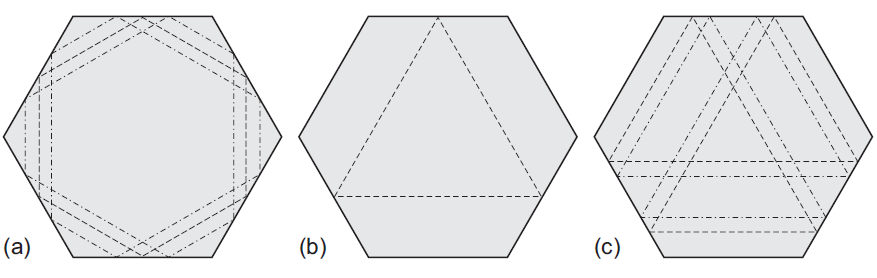
\includegraphics[width=.7\textwidth]{Bilder/wgm}
\caption[Whispering-Gallery-Moden]{Schematische Darstellung der Whispering-Gallery-Moden a) hexagonal 6WG-Moden (gestrichelt symmetische Mode, strichpunktiert zwei nichtsymmetrische)b) 3WG-Mode sowie c) zwei verschiedene D3-WG-Moden (eine gestrichelt, die andere strichpunktiert)\cite{Grundmann.2012}}
\label{WGM}
\end{figure}

Mit Hilfe eines Rasterelektronenmikroskops (s. \autoref{RKM}) wird die Qualität der Drähte beurteilt, Proben ohne die gewünschten charakteristischen Nanodrähte werden verworfen.\\
\begin{table}
\begin{tabular}{llll}
Wachstumsdruck p & Temperatur $\text{T}_\text{max}$ & Wachstumszeit $\text{t}_\text{w}$ & Ar-Volumenfluss $\text{q}_\text{Ar}$ \\ 
100 mbar & 1350 $^{\circ}$C & 60 min & 50 sccm \\ 
\end{tabular}
\caption[VLS-Wachstumsparameter]{Die wichtigsten Wachstumsparameter der Drahtsynthese} 
\end{table}